% Options for packages loaded elsewhere
\PassOptionsToPackage{unicode}{hyperref}
\PassOptionsToPackage{hyphens}{url}
%
\documentclass[
]{book}
\usepackage{amsmath,amssymb}
\usepackage{lmodern}
\usepackage{ifxetex,ifluatex}
\ifnum 0\ifxetex 1\fi\ifluatex 1\fi=0 % if pdftex
  \usepackage[T1]{fontenc}
  \usepackage[utf8]{inputenc}
  \usepackage{textcomp} % provide euro and other symbols
\else % if luatex or xetex
  \usepackage{unicode-math}
  \defaultfontfeatures{Scale=MatchLowercase}
  \defaultfontfeatures[\rmfamily]{Ligatures=TeX,Scale=1}
\fi
% Use upquote if available, for straight quotes in verbatim environments
\IfFileExists{upquote.sty}{\usepackage{upquote}}{}
\IfFileExists{microtype.sty}{% use microtype if available
  \usepackage[]{microtype}
  \UseMicrotypeSet[protrusion]{basicmath} % disable protrusion for tt fonts
}{}
\makeatletter
\@ifundefined{KOMAClassName}{% if non-KOMA class
  \IfFileExists{parskip.sty}{%
    \usepackage{parskip}
  }{% else
    \setlength{\parindent}{0pt}
    \setlength{\parskip}{6pt plus 2pt minus 1pt}}
}{% if KOMA class
  \KOMAoptions{parskip=half}}
\makeatother
\usepackage{xcolor}
\IfFileExists{xurl.sty}{\usepackage{xurl}}{} % add URL line breaks if available
\IfFileExists{bookmark.sty}{\usepackage{bookmark}}{\usepackage{hyperref}}
\hypersetup{
  pdftitle={写给文科生的Python入门和数据处理教程},
  pdfauthor={Li Weicheng @ gpnu},
  hidelinks,
  pdfcreator={LaTeX via pandoc}}
\urlstyle{same} % disable monospaced font for URLs
\usepackage{color}
\usepackage{fancyvrb}
\newcommand{\VerbBar}{|}
\newcommand{\VERB}{\Verb[commandchars=\\\{\}]}
\DefineVerbatimEnvironment{Highlighting}{Verbatim}{commandchars=\\\{\}}
% Add ',fontsize=\small' for more characters per line
\usepackage{framed}
\definecolor{shadecolor}{RGB}{248,248,248}
\newenvironment{Shaded}{\begin{snugshade}}{\end{snugshade}}
\newcommand{\AlertTok}[1]{\textcolor[rgb]{0.94,0.16,0.16}{#1}}
\newcommand{\AnnotationTok}[1]{\textcolor[rgb]{0.56,0.35,0.01}{\textbf{\textit{#1}}}}
\newcommand{\AttributeTok}[1]{\textcolor[rgb]{0.77,0.63,0.00}{#1}}
\newcommand{\BaseNTok}[1]{\textcolor[rgb]{0.00,0.00,0.81}{#1}}
\newcommand{\BuiltInTok}[1]{#1}
\newcommand{\CharTok}[1]{\textcolor[rgb]{0.31,0.60,0.02}{#1}}
\newcommand{\CommentTok}[1]{\textcolor[rgb]{0.56,0.35,0.01}{\textit{#1}}}
\newcommand{\CommentVarTok}[1]{\textcolor[rgb]{0.56,0.35,0.01}{\textbf{\textit{#1}}}}
\newcommand{\ConstantTok}[1]{\textcolor[rgb]{0.00,0.00,0.00}{#1}}
\newcommand{\ControlFlowTok}[1]{\textcolor[rgb]{0.13,0.29,0.53}{\textbf{#1}}}
\newcommand{\DataTypeTok}[1]{\textcolor[rgb]{0.13,0.29,0.53}{#1}}
\newcommand{\DecValTok}[1]{\textcolor[rgb]{0.00,0.00,0.81}{#1}}
\newcommand{\DocumentationTok}[1]{\textcolor[rgb]{0.56,0.35,0.01}{\textbf{\textit{#1}}}}
\newcommand{\ErrorTok}[1]{\textcolor[rgb]{0.64,0.00,0.00}{\textbf{#1}}}
\newcommand{\ExtensionTok}[1]{#1}
\newcommand{\FloatTok}[1]{\textcolor[rgb]{0.00,0.00,0.81}{#1}}
\newcommand{\FunctionTok}[1]{\textcolor[rgb]{0.00,0.00,0.00}{#1}}
\newcommand{\ImportTok}[1]{#1}
\newcommand{\InformationTok}[1]{\textcolor[rgb]{0.56,0.35,0.01}{\textbf{\textit{#1}}}}
\newcommand{\KeywordTok}[1]{\textcolor[rgb]{0.13,0.29,0.53}{\textbf{#1}}}
\newcommand{\NormalTok}[1]{#1}
\newcommand{\OperatorTok}[1]{\textcolor[rgb]{0.81,0.36,0.00}{\textbf{#1}}}
\newcommand{\OtherTok}[1]{\textcolor[rgb]{0.56,0.35,0.01}{#1}}
\newcommand{\PreprocessorTok}[1]{\textcolor[rgb]{0.56,0.35,0.01}{\textit{#1}}}
\newcommand{\RegionMarkerTok}[1]{#1}
\newcommand{\SpecialCharTok}[1]{\textcolor[rgb]{0.00,0.00,0.00}{#1}}
\newcommand{\SpecialStringTok}[1]{\textcolor[rgb]{0.31,0.60,0.02}{#1}}
\newcommand{\StringTok}[1]{\textcolor[rgb]{0.31,0.60,0.02}{#1}}
\newcommand{\VariableTok}[1]{\textcolor[rgb]{0.00,0.00,0.00}{#1}}
\newcommand{\VerbatimStringTok}[1]{\textcolor[rgb]{0.31,0.60,0.02}{#1}}
\newcommand{\WarningTok}[1]{\textcolor[rgb]{0.56,0.35,0.01}{\textbf{\textit{#1}}}}
\usepackage{longtable,booktabs,array}
\usepackage{calc} % for calculating minipage widths
% Correct order of tables after \paragraph or \subparagraph
\usepackage{etoolbox}
\makeatletter
\patchcmd\longtable{\par}{\if@noskipsec\mbox{}\fi\par}{}{}
\makeatother
% Allow footnotes in longtable head/foot
\IfFileExists{footnotehyper.sty}{\usepackage{footnotehyper}}{\usepackage{footnote}}
\makesavenoteenv{longtable}
\usepackage{graphicx}
\makeatletter
\def\maxwidth{\ifdim\Gin@nat@width>\linewidth\linewidth\else\Gin@nat@width\fi}
\def\maxheight{\ifdim\Gin@nat@height>\textheight\textheight\else\Gin@nat@height\fi}
\makeatother
% Scale images if necessary, so that they will not overflow the page
% margins by default, and it is still possible to overwrite the defaults
% using explicit options in \includegraphics[width, height, ...]{}
\setkeys{Gin}{width=\maxwidth,height=\maxheight,keepaspectratio}
% Set default figure placement to htbp
\makeatletter
\def\fps@figure{htbp}
\makeatother
\setlength{\emergencystretch}{3em} % prevent overfull lines
\providecommand{\tightlist}{%
  \setlength{\itemsep}{0pt}\setlength{\parskip}{0pt}}
\setcounter{secnumdepth}{5}
\usepackage{booktabs}
\ifluatex
  \usepackage{selnolig}  % disable illegal ligatures
\fi
\usepackage[]{natbib}
\bibliographystyle{plainnat}

\title{写给文科生的Python入门和数据处理教程}
\author{Li Weicheng @ gpnu}
\date{2021-09-07}

\begin{document}
\maketitle

{
\setcounter{tocdepth}{1}
\tableofcontents
}
\begin{Shaded}
\begin{Highlighting}[]
\NormalTok{colorize }\OtherTok{\textless{}{-}} \ControlFlowTok{function}\NormalTok{(x, color) \{}
  \ControlFlowTok{if}\NormalTok{ (knitr}\SpecialCharTok{::}\FunctionTok{is\_latex\_output}\NormalTok{()) \{}
    \FunctionTok{sprintf}\NormalTok{(}\StringTok{"}\SpecialCharTok{\textbackslash{}\textbackslash{}}\StringTok{textcolor\{\%s\}\{\%s\}"}\NormalTok{, color, x)}
\NormalTok{  \} }\ControlFlowTok{else} \ControlFlowTok{if}\NormalTok{ (knitr}\SpecialCharTok{::}\FunctionTok{is\_html\_output}\NormalTok{()) \{}
    \FunctionTok{sprintf}\NormalTok{(}\StringTok{"\textless{}span style=\textquotesingle{}color: \%s;\textquotesingle{}\textgreater{}\%s\textless{}/span\textgreater{}"}\NormalTok{, color,}
\NormalTok{      x)}
\NormalTok{  \} }\ControlFlowTok{else}\NormalTok{ x}
\NormalTok{\}}
\end{Highlighting}
\end{Shaded}

\hypertarget{ux5f15ux8a00}{%
\chapter{引言}\label{ux5f15ux8a00}}

本文是Python入门和数据处理教程,基于经管类本科课堂教学用的讲义,以供同学们自学和参考。

\emph{p.s.} 本文使用RStudio以及R的Bookdown包写成。

\hypertarget{ux672cux4e66ux76eeux6807}{%
\section{本书目标}\label{ux672cux4e66ux76eeux6807}}

\begin{enumerate}
\def\labelenumi{\arabic{enumi}.}
\tightlist
\item
  负基础Python入门
\end{enumerate}

对于首次接触编程的人,可能对计算机和操作系统的有关知识(如``命令行'',``路径''等)缺乏了解。本文尽量把有关的知识都介绍到,争取做到``会打字就能学Python''。

\begin{enumerate}
\def\labelenumi{\arabic{enumi}.}
\setcounter{enumi}{1}
\tightlist
\item
  Python数据处理
\end{enumerate}

\begin{itemize}
\tightlist
\item
  基本目标:替代Excel
\item
  进阶目标:对科研常用数据,如Wind和CSMAR数据库、CFPS和CHIP等微观调查数据、统计局数据、oTree实验数据等,按照研究要求进行清洗、剪裁、整合以及绘图,为进一步分析(如回归)制作出合适的数据集。
\end{itemize}

\begin{enumerate}
\def\labelenumi{\arabic{enumi}.}
\setcounter{enumi}{2}
\tightlist
\item
  金融数据分析
\end{enumerate}

待定:视教学情况。

\hypertarget{ux672cux4e66ux4e0dux8db3}{%
\section{本书不足}\label{ux672cux4e66ux4e0dux8db3}}

\begin{enumerate}
\def\labelenumi{\arabic{enumi}.}
\tightlist
\item
  由于课时非常紧张,有很多有意义的内容不得不舍弃,包括但不限于:
\end{enumerate}

\begin{itemize}
\tightlist
\item
  函数式编程和数据流思想
\item
  面向对象编程
\item
  单元测试
\end{itemize}

\begin{enumerate}
\def\labelenumi{\arabic{enumi}.}
\setcounter{enumi}{1}
\tightlist
\item
  作者水平有限,很多内容未必是最优做法,只能争取尽量清晰和明确。
\item
  要顾及同学们的计算机基础有高有低,有些地方不得不写得比较啰嗦。
\end{enumerate}

\hypertarget{ux4f7fux7528ux7684ux7a0bux5e8fux548cux7248ux672c}{%
\section{使用的程序和版本}\label{ux4f7fux7528ux7684ux7a0bux5e8fux548cux7248ux672c}}

\begin{enumerate}
\def\labelenumi{\arabic{enumi}.}
\tightlist
\item
  使用Anaconda以及附带的Spyder作为主要的编程环境
\item
  Python版本3.6或以上。(涉及Type Hints和f-string等)
\end{enumerate}

\hypertarget{ux628apythonux5b89ux88c5ux5230ux4f60ux7684ux7535ux8111ux91cc}{%
\section{把Python安装到你的电脑里}\label{ux628apythonux5b89ux88c5ux5230ux4f60ux7684ux7535ux8111ux91cc}}

要完成任何一个编程任务,首先要借助Python现有的巨大的程序库(一般可称为库Library,或者包Package)。本课程主要针对经济类数据分析,涉及的包比较多。为了避免逐个安装,我们采用比较简单的做法,直接安装Anaconda。这是一个所谓``Python发行版'',里面包含了Python的执行程序(解释器等),以及大量的科学计算用包。一般的数据分析工作,直接安装这个即可。

下载地址:\url{https://www.anaconda.com/products/individual\#Downloads}

直接百度Anaconda也能找到这个链接。按照你自己的操作系统下载 ,一般选择\textbf{最新版},现在的电脑一般选择\textbf{64bit}的安装文件,安装过程采用\textbf{默认选项}即可。

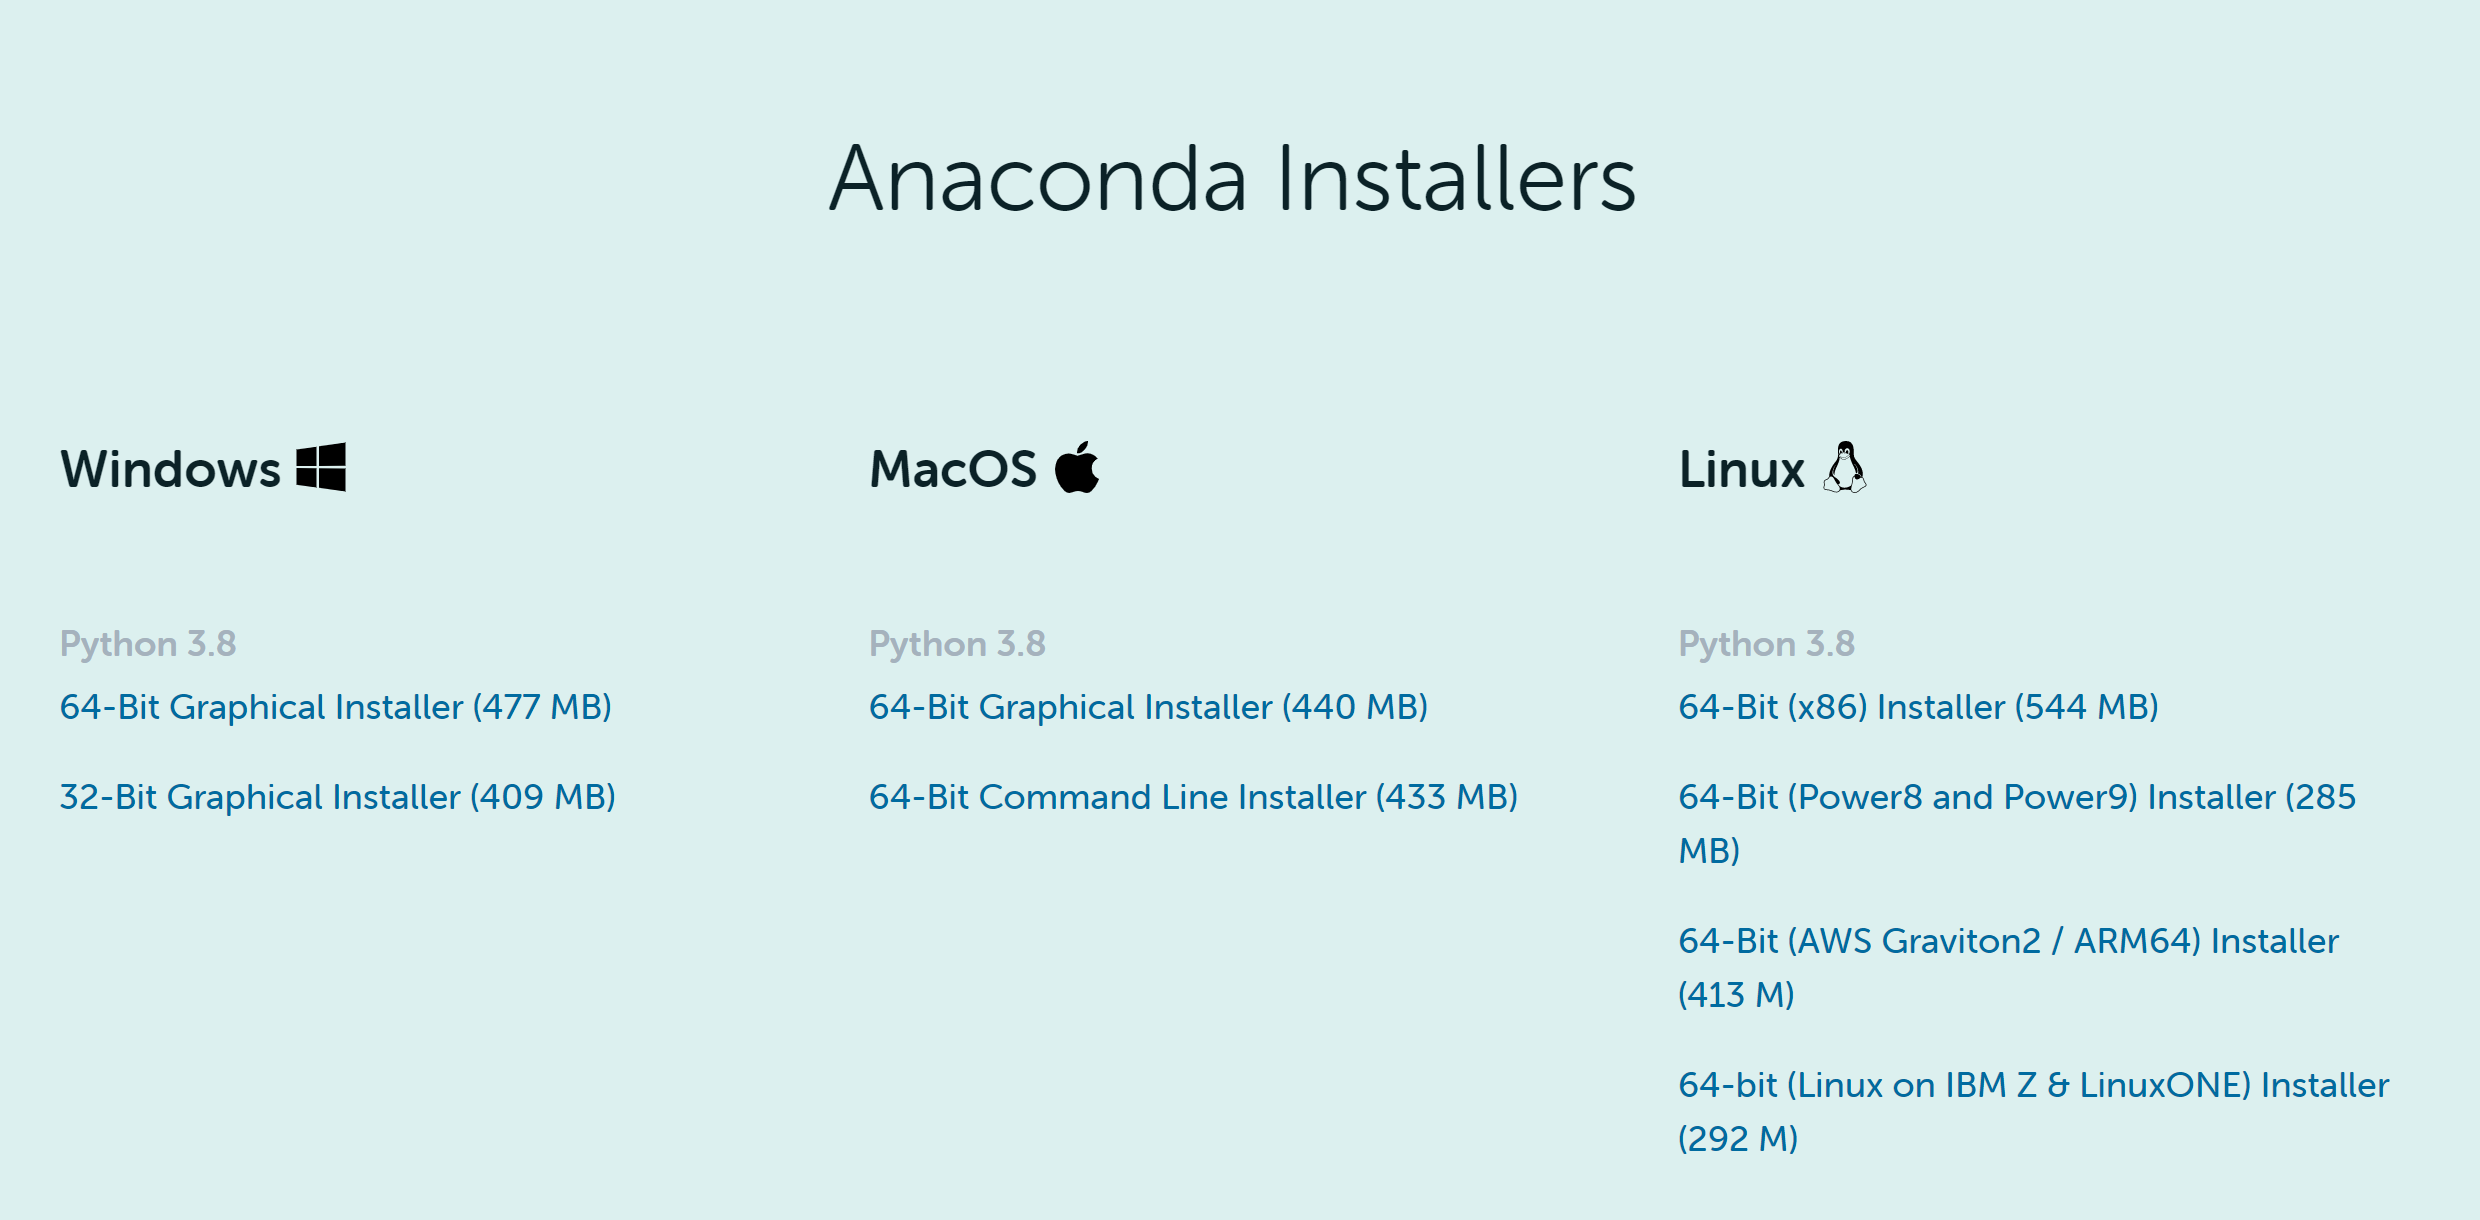
\includegraphics{images/anaconda_download.png}

\hypertarget{pythonux7a0bux5e8fux7684ux6267ux884c}{%
\chapter{Python程序的执行}\label{pythonux7a0bux5e8fux7684ux6267ux884c}}

\hypertarget{ux4e00ux4e2apythonux7a0bux5e8fux662fux4ec0ux4e48}{%
\section{一个Python程序是什么}\label{ux4e00ux4e2apythonux7a0bux5e8fux662fux4ec0ux4e48}}

我们所谓``写一个Python''程序,到底是在写一个什么东西?

一般情况下,所谓一个Python程序,仅仅是一个你电脑里的\textbf{纯文本文件},但\protect\hyperlink{ext_name}{扩展名}是\texttt{*.py},这个文件本质上一个\texttt{.txt}文件没什么不同,都可以用任何文本编辑器(例如你电脑里的``记事本'')打开和编辑。

我们要做的工作,就是用一个文本编辑器(当然也可以是一个集成编程环境如后面会用到的Spyder),编辑一个\texttt{.py}文件,然后把你要的代码写进去,用不同的方法去执行这个文件里代码。可能是在系统里一次性执行整个文件里所有代码,也可能是在一个交互环境里一步一步地执行。

\hypertarget{ext_name}{%
\subsection{基础知识:扩展名和文件类型}\label{ext_name}}

用于表示某个文件是什么类型,一般我们会看文件名的最后一个英文\texttt{.}以及之后的内容。

\textbf{注意}:这里只是泛泛而论。扩展名也是可以修改的,所以未必和实际的文件类型一致。

\begin{enumerate}
\def\labelenumi{\arabic{enumi}.}
\tightlist
\item
  一个文件,其名为\texttt{WINWORD.EXE},其扩展名为\texttt{.exe}(Window系统的文件名不区分大小写,但Mac系统的文件名严格区分大小写),则意味着这是一个``Windows系统的可执行文件''。这实际上是微软Windows版本office中的Word的主程序。我们(在windows下)常说的``运行一个程序'',就是执行一个exe文件。
\item
  一个文件,其名为\texttt{鲁迅全集.txt},其扩展名为\texttt{.txt},则意味着这是一个``纯文本文件'',其中的所有内容都可以视为文字,可以用任何一个文本编辑器,例如记事本,或者Word打开。
\item
  其他扩展名,如\texttt{.jpg}是常见的图形文件,\texttt{.docx}是2007版本以后的Word文档,等等等等。
\end{enumerate}

\hypertarget{python_interactive}{%
\section{Python的交互式环境}\label{python_interactive}}

我们先采用最基本的Python的交互式环境,给大家一点运行程序的感觉。

\begin{enumerate}
\def\labelenumi{\arabic{enumi}.}
\tightlist
\item
  启动Anaconda Prompt。(用Mac的同学,启动终端terminal)
\end{enumerate}

\begin{enumerate}
\def\labelenumi{\arabic{enumi}.}
\setcounter{enumi}{1}
\tightlist
\item
  我们会看到命令行窗口
\end{enumerate}

\begin{enumerate}
\def\labelenumi{\arabic{enumi}.}
\setcounter{enumi}{2}
\tightlist
\item
  输入\texttt{python\ \textless{}回车\textgreater{}},我们可以进入python的交互式运行环境。
\end{enumerate}

{\textbf{注意:}}
其中的命令提示符\texttt{\textgreater{}\textgreater{}\textgreater{}}。三个右侧尖括号,表示\textbf{我们正处于python的交互式环境中},此时我们可以执行python的语句。

同时可见Python的版本为3.9.5,一般3.7.x以上皆可。

\hypertarget{ux7b80ux5355ux7684ux7f16ux7a0bux8ba1ux7b971-2}{%
\subsection{简单的编程:计算1 + 2}\label{ux7b80ux5355ux7684ux7f16ux7a0bux8ba1ux7b971-2}}

\begin{enumerate}
\def\labelenumi{\arabic{enumi}.}
\tightlist
\item
  我们依次输入(每行代码以结束)
\end{enumerate}

\begin{verbatim}
>>> a = 1
>>> b = 2
>>> c = a + b 
>>> print(c)
\end{verbatim}

显然,1+2必然得到

\begin{verbatim}
3
\end{verbatim}

\begin{enumerate}
\def\labelenumi{\arabic{enumi}.}
\setcounter{enumi}{1}
\tightlist
\item
  结果大致如图
\end{enumerate}

{\textbf{注意:}}

\begin{itemize}
\tightlist
\item
  无法得到结果\texttt{3},首先检查有没有\textbf{输入错误(打错字)}。
\item
  \texttt{print(c)}中的小括号,是英文括号。在语法层面上的所有符号,都是\textbf{英文符号}。
\item
  如果输入的代码有误,已经敲了回车,只要把正确代码的再输入一次即可。
\end{itemize}

\hypertarget{ux4e0aux8ff0ux7a0bux5e8fux4e2dux6d89ux53caux7684ux4e00ux4e9bux6982ux5ff5}{%
\subsection{上述程序中涉及的一些概念}\label{ux4e0aux8ff0ux7a0bux5e8fux4e2dux6d89ux53caux7684ux4e00ux4e9bux6982ux5ff5}}

这个涉及程序设计的几个基本概念:

\begin{enumerate}
\def\labelenumi{\arabic{enumi}.}
\tightlist
\item
  变量和赋值
\end{enumerate}

变量,顾名思义,一个可变的量。编程中变量的概念和代数中的\texttt{x}, \texttt{y}, \texttt{z}基本一样。
Python中,对变量赋值使用1个等号 ``\texttt{=}''。
显然, 我们有3个变量,\texttt{a}, \texttt{b}和\texttt{c}。我们把\texttt{1}赋予\texttt{a},\texttt{2}赋予\texttt{b},把\texttt{a\ +\ b}的值赋予\texttt{c}。

\begin{enumerate}
\def\labelenumi{\arabic{enumi}.}
\setcounter{enumi}{1}
\tightlist
\item
  运算符
\end{enumerate}

加减乘除,以及逻辑运算如是否等于,大于,小于等,我们以后会用到。这里只用到``加法''

\begin{enumerate}
\def\labelenumi{\arabic{enumi}.}
\setcounter{enumi}{2}
\tightlist
\item
  函数
\end{enumerate}

和数学函数一样,我们调用一个函数,给这个函数传递一个参数,然后这个函数会根据这个参数做一些事情。可能是为你进行一个计算,可能修改某个变量等等,也可能什么都不做。

这里我们调用的函数是\texttt{print()},这个函数的用途是把你传递给他的变量\texttt{c}的值打印出来。函数的调用方法是函数名与小括号。

\textbf{数据分析的程序,大部分情况下可以视为由变量和函数组成。}

\hypertarget{ux9000ux51faux8fd0ux884cux73afux5883}{%
\subsection{退出运行环境}\label{ux9000ux51faux8fd0ux884cux73afux5883}}

输入\texttt{exit()},然后回车即可。

可见,\texttt{exit}本身也是一个函数(函数名+小括号),其调用这个函数的作用是退出Python交互式运行环境。

{\textbf{注意:}}一定要退出,以便后续的程序能执行。

此时,我们又回到了一开始的命令行(终端)环境中

可见,命令提示符现在是一个\texttt{\textgreater{}},这提示我们正处于系统的命令行环境中

\begin{enumerate}
\def\labelenumi{\arabic{enumi}.}
\tightlist
\item
  可以执行系统中的命令,但不能执行python中的语句!
\item
  要进行交互式的python编程,要首先进入\protect\hyperlink{python_interactive}{Python的交互式环境}中!
\end{enumerate}

\hypertarget{ux9884ux5907ux77e5ux8bc6ux8defux5f84}{%
\section{预备知识:路径}\label{ux9884ux5907ux77e5ux8bc6ux8defux5f84}}

\hypertarget{path}{%
\subsection{路径Path}\label{path}}

\emph{你的文件或者文件夹(目录),到底保存到了哪里?}

所谓路径(path),到达某个文件或者文件夹(目录)的层级结构,每一层用一个斜杠``\texttt{/}''分割。

在命令行(终端)环境下,在命令提示符\texttt{\textgreater{}}之前,一般会有提示你当前路径,即当前你处于哪个目录下。

例如 \texttt{C:\textbackslash{}Users\textbackslash{}lee},指的就是,在你的\texttt{C}盘下,\texttt{Users}目录下,的\texttt{lee}目录。

{\textbf{注意:}}在你的电脑上,这里的\texttt{lee}会替换为你的用户名

这样,你输入的任何命令,都会对``当前路径''生效。

同样,路径既可以指向一个目录(文件夹),也可以指向一个文件。

如\texttt{C:\textbackslash{}Users\textbackslash{}lee\textbackslash{}add.py},就指的是,在你的\texttt{C}盘下的\texttt{Users}目录下的\texttt{lee}目录下的一个叫\texttt{add.py}的文件。

\hypertarget{ux76f8ux5bf9ux8defux5f84ux548cux7eddux5bf9ux8defux5f84}{%
\subsection{相对路径和绝对路径}\label{ux76f8ux5bf9ux8defux5f84ux548cux7eddux5bf9ux8defux5f84}}

\begin{enumerate}
\def\labelenumi{\arabic{enumi}.}
\tightlist
\item
  绝对路径:从根目录(windows下即一个盘符,如c盘或者d盘)开始的路径,可以确定无疑地指向某个文件或者目录。如\texttt{C:\textbackslash{}Users\textbackslash{}lee\textbackslash{}add.py}。
\item
  相对路径:不从根目录起始的路径。其指向的目的地,从你的``当前路径''开始,往下数。
\end{enumerate}

假如,你的当前路径是\texttt{C:\textbackslash{}Users},那么此时,相对路径\texttt{lee\textbackslash{}add.py},所指向的,就是当前路径下(\texttt{C:\textbackslash{}Users}),\texttt{lee}目录下的\texttt{add.py}。这也等价于绝对路径\texttt{C:\textbackslash{}Users\textbackslash{}lee\textbackslash{}add.py}。

\begin{enumerate}
\def\labelenumi{\arabic{enumi}.}
\setcounter{enumi}{2}
\tightlist
\item
  两者的区别:绝对路径从根目录开始,相对路径从``当前路径''开始。
\end{enumerate}

\hypertarget{ux8fdbux5165ux67d0ux4e2aux76eeux5f55}{%
\subsection{进入某个目录}\label{ux8fdbux5165ux67d0ux4e2aux76eeux5f55}}

Windows命令行,和Mac的终端,有相同的命令\texttt{cd\ \textless{}路径\textgreater{}},可以进入一个目录。

如,在终端中输入(并回车)注意这里使用的是绝对路径

\begin{verbatim}
cd C:/Users 
\end{verbatim}

则会让终端进入到 \texttt{C:/Users} 目录下。见提示符\texttt{\textgreater{}}前方的``当前路径''已经改变为\texttt{C:/Users}。你现在已经位于\texttt{C:/Users} 目录。

尝试相对路径,在终端中输入(并回车),注意这里的\texttt{lee},请替换成你的用户名。

\begin{verbatim}
cd lee
\end{verbatim}

则会让终端进入到 \texttt{C:/Users/lee} 目录下。见提示符\texttt{\textgreater{}}前方的``当前路径''已经改变为\texttt{C:/Users/lee}。你现在已经位于\texttt{C:/Users/lee} 目录。

其他用法包括:

\begin{enumerate}
\def\labelenumi{\arabic{enumi}.}
\tightlist
\item
  进入上一级目录
\end{enumerate}

\begin{verbatim}
cd ..
\end{verbatim}

\begin{enumerate}
\def\labelenumi{\arabic{enumi}.}
\setcounter{enumi}{1}
\tightlist
\item
  进入根目录
\end{enumerate}

\begin{verbatim}
cd /
\end{verbatim}

可以让你在命令行和终端中,定位到你想要的目录和文件。

\hypertarget{use_win}{%
\subsection{用Windows图形界面获得路径}\label{use_win}}

在你的windows资源管理器(俗称``我的电脑''),在任何一个文件夹中,点击地址栏

你就可以得到这个文件夹的路径,可以粘贴到命令行中。

{\textbf{特别注意:正反斜杠问题}}

在编程的语境下,反斜杠``\texttt{\textbackslash{}}''有特殊用途。因此,表示路径的时候,我们统一用(正)斜杠``\texttt{/}'',而不用反斜杠``\texttt{\textbackslash{}}''。

统一的写法,如\texttt{C:/Users/lee}

\hypertarget{ux5217ux76eeux5f55}{%
\subsection{列目录}\label{ux5217ux76eeux5f55}}

列目录的命令,Windows的命令行中为\texttt{dir},Mac中为\texttt{ls}。同学们可以执行尝试。

\hypertarget{ux7528pythonux89e3ux91caux5668ux6765ux8fd0ux884c}{%
\section{用Python解释器来运行}\label{ux7528pythonux89e3ux91caux5668ux6765ux8fd0ux884c}}

当你离开交互环境,你的程序就没了。当然,我们不可能每次都把程序从头写一次。如前文所述,我们编写一个\texttt{.py}文件来保存我们的代码,然后利用系统中安装的Python解释器来执行它。

\hypertarget{ux7f16ux5199ux6e90ux4ee3ux7801}{%
\subsection{编写源代码}\label{ux7f16ux5199ux6e90ux4ee3ux7801}}

前面说过,python的代码文件\texttt{.py}是一个和\texttt{.txt}同样的纯文本文件,所以我们这次直接用记事本来编辑。

打开windows的记事本,把刚才的1 + 2程序写进去,按ctrl+s保存

\begin{Shaded}
\begin{Highlighting}[]
\NormalTok{a }\OperatorTok{=} \DecValTok{1}
\NormalTok{b }\OperatorTok{=} \DecValTok{2}
\NormalTok{c }\OperatorTok{=}\NormalTok{ a }\OperatorTok{+}\NormalTok{ b}
\BuiltInTok{print}\NormalTok{(c)}
\end{Highlighting}
\end{Shaded}

\begin{enumerate}
\def\labelenumi{\arabic{enumi}.}
\tightlist
\item
  在\texttt{C}盘根目录下,建立一个新的文件夹,例如``\texttt{PythonClass}''。
\item
  类型选择\emph{.}(所有文件),文件名可以任意起,但是必须以\texttt{.py}结尾。例如我这里采用\texttt{add.py}。
\item
  保存。
\end{enumerate}

注意:

\begin{enumerate}
\def\labelenumi{\arabic{enumi}.}
\tightlist
\item
  如果你按此操作,那么你的\texttt{PythonClass}文件夹的完整路径(绝对路径)就是\texttt{C:/PythonClass}。而你的\texttt{.py}文件的完整路径,就是\texttt{C:/PythonClass/add.py}
\item
  如果你自行选取其他位置保存\texttt{.py}文件,那么路径也可以如此类推。如果实在找不到,则可见\protect\hyperlink{use_win}{在Windows图形界面获得路径}。
\end{enumerate}

\hypertarget{ux6267ux884cux8fd9ux4e2aux4ee3ux7801}{%
\subsection{执行这个代码}\label{ux6267ux884cux8fd9ux4e2aux4ee3ux7801}}

确保你刚才已经退出了Python的交互环境。我们现在首先要定位到我们保存\texttt{.py}文件的目录,如果大家按操作运行,这个文件应该在\texttt{C:/PythonClass}目录下。
我们\texttt{cd}命令,转移到我们保存\texttt{py}文件的路径:

输入 (并回车)

\begin{verbatim}
cd C:/PythonClass
\end{verbatim}

此时你的命令提示符应该告诉你,现在位于\texttt{C:/PythonClass}目录下。

\begin{verbatim}
C:\PythonClass>_
\end{verbatim}

输入(并回车)

\begin{verbatim}
python add.py
\end{verbatim}

这句命令的含义是:让系统中装好的python解释器,去运行\texttt{add.py}这个python脚本文件。这个脚本文件就在当前目录中(或者环境变量path中的目录,现在可以忽略这一点)。

实际上,我们以用绝对路径来指向\texttt{add.py},也是一样的。

\begin{verbatim}
python C:/PythonClass/add.py
\end{verbatim}

如果一切顺利,你将会看到结果

\begin{verbatim}
3
\end{verbatim}

而不同之处在于,我们的程序这次保留了下来,我们要继续上一次编程,我们只要打开这个py文件,继续往里写代码即可。

那如果我们既要保存代码,又要一边执行代码、一边看结果怎么办?

\hypertarget{ux4f7fux7528spyderux7f16ux7a0bux73afux5883}{%
\chapter{使用Spyder编程环境}\label{ux4f7fux7528spyderux7f16ux7a0bux73afux5883}}

实际上,我们真正用python做数据分析的时候,一般会利用一个集成编程环境,例如我们\textbf{本课程要用的Spyder},或者流行的PyCharm,或者jupyter notebook等等。

这些集成编辑环境,通常会把.py文件的编辑和python的交互环境结合起来,让我们一边编辑py文件的同时,一边执行代码并查看结果。数据分析完毕时,代码同时也写成了。

\hypertarget{ux754cux9762}{%
\section{界面}\label{ux754cux9762}}

打开Spyder

Spyder默认打开了一个临时的\texttt{.py}文件。

\begin{enumerate}
\def\labelenumi{\arabic{enumi}.}
\tightlist
\item
  左边是一个\textbf{文本编辑器}(回忆前面我们编辑\texttt{add.py}文件所用的\textbf{记事本})。
\item
  文本编辑器的标签页,显示我们当前打开的文件是\texttt{temp.py}。如果文件名后带\texttt{*}号,表示这个文件修改了但尚未保存。
\item
  标签页上方,显示了当前文件\texttt{temp.py}的\protect\hyperlink{path}{路径}。显然,这是一个绝对路径,显示了从根目录开始到这个文件的完整路径。
\item
  右下角是Python的交互运行环境。这个环境叫\texttt{IPython},比我们刚才运行\protect\hyperlink{python_interactive}{Python交互环境}要稍微先进一点,但本质上并无不同。
\item
  工具栏,我们后面再说。
\end{enumerate}

\hypertarget{ux5728spyderux4e2dux5199ux4ee3ux7801}{%
\section{在Spyder中写代码}\label{ux5728spyderux4e2dux5199ux4ee3ux7801}}

我们在左侧的文本编辑器,把刚才的1+2程序写进去,按Ctrl+s保存一下(Mac: Cmd + s)。

\hypertarget{ux8fd0ux884cux7a0bux5e8f}{%
\section{运行程序}\label{ux8fd0ux884cux7a0bux5e8f}}

\hypertarget{ux4eceux5934ux5230ux5c3eux8fd0ux884cux4ee3ux7801}{%
\subsection{从头到尾运行代码}\label{ux4eceux5934ux5230ux5c3eux8fd0ux884cux4ee3ux7801}}

点击工具栏的运行按钮(Run File),或者按键盘的F5,我们可以把当前的\texttt{.py}脚本从头到尾运行一遍。
看交互式窗口,得到结果为\texttt{3}。

Run File,这个按钮的功能约等于我们在命令行环境下,直接运行``\texttt{Python\ temp.py}''。(注意我们正在编辑的文件是\texttt{temp.py})

\hypertarget{ux53d8ux91cfux76d1ux89c6ux5668}{%
\subsection{变量监视器}\label{ux53d8ux91cfux76d1ux89c6ux5668}}

点击右上角一栏的\texttt{Variable\ Explorer}(变量浏览器),可以看到当前运行环境中的所有变量和他们的类型以及值(变量类型见后)。
点击交互界面上方的垃圾桶图标\texttt{Remove\ all\ variables}(移除所有变量),点击yes。

\hypertarget{ux5355ux6b65ux6267ux884c}{%
\subsection{单步执行}\label{ux5355ux6b65ux6267ux884c}}

现在找到``Run selection or current line''按钮。

这个按钮,顾名思义。如果你选择了一部分代码则,执行这部分代码。如果你没有选择代码,则执行光标所在行。执行完毕后,光标会自动移动到下一行。

让我们试一下。

\begin{enumerate}
\def\labelenumi{\arabic{enumi}.}
\tightlist
\item
  点击第一行a=1,让输入光标在这一行
\item
  点击 ,或者F9
\item
  我们可以看到,这个按钮把光标所在行的代码``a = 1'',发送到了交互窗口,并执行,且光标自动下移了一行。
\item
  右上方的变量浏览器,现在自动出现了变量a
\end{enumerate}

显然,如果我们连续点击,或者连按F9,我们就可以连续地、单步执行代码。每按一次,Spyder会把当前行的代码(或者你选定的代码),发送到交互窗口并执行。

打一个比方,这就像你同时打开记事本和python交互环境,一边在记事本中写代码,一边手动地拷贝粘贴到python交互环境中执行,是同样的逻辑。

这使得我们可以逐步查看每一行代码的效果,是实际工作中的常规操作之一。

\hypertarget{ux9009ux62e9ux6267ux884c}{%
\subsection{选择执行}\label{ux9009ux62e9ux6267ux884c}}

这个按钮也可以一次性执行\textbf{你所选择的代码},这个大家可以自行尝试。

\hypertarget{ux9884ux5907ux77e5ux8bc6pythonux7684ux6ce8ux91cacomment}{%
\section{预备知识:Python的注释(comment)}\label{ux9884ux5907ux77e5ux8bc6pythonux7684ux6ce8ux91cacomment}}

先说注释。Python使用井号:\texttt{\#}来表示注释。所谓注释,就是``\textbf{给人看}''的内容,而Python的解释器会直接忽略掉这部分。

\begin{enumerate}
\def\labelenumi{\arabic{enumi}.}
\tightlist
\item
  注释可以出现在任何地方,注意\texttt{\#}号只会影响同一行右边的代码,因此也可以出现在行尾。
\item
  注释往往也可以用来临时屏蔽一部分代码,只要在代码的最左侧插入一个\texttt{\#},那么整行代码会被Python解释器忽略。这是常用技巧。
\end{enumerate}

我们尝试写几个注释,例如:

注释是对代码的说明,非常重要:

\begin{enumerate}
\def\labelenumi{\arabic{enumi}.}
\tightlist
\item
  写代码时间长了,肯定会不记得自己写的内容。有时候上午写的,下午就会忘记。
\item
  多人合作的时候,要读懂彼此的代码,也必须有良好的注释。
\end{enumerate}

特别地,\textbf{注释是考试的给分点}。你的考试程序输出了正确的结果,可以得到合格评价,同时具有良好的编写风格、合理的注释,才能得到更高分。

\hypertarget{ux8fd0ux884cux7a0bux5e8fux7eed}{%
\section{运行程序(续)}\label{ux8fd0ux884cux7a0bux5e8fux7eed}}

\hypertarget{ux6309cellux5355ux5143ux683cux6267ux884c}{%
\subsection{按Cell(单元格)执行}\label{ux6309cellux5355ux5143ux683cux6267ux884c}}

一般我们的程序,往往有一长串代码,或者连续几条语句,只是为了达到某一个特定目的。如果我们修改了某些代码,希望把整个代码块一次执行完,直接查看阶段性的结果,就可以使用cell。

可以使用特殊的注释\texttt{\#\%\%},两个\texttt{\#\%\%}中间的代码,会被Spyder认为是一个cell(单元格)。光标所在的cell,会有不同颜色的背景颜色来区分。

定义好cell之后,我们可以使用工具栏中的2个按钮

\begin{enumerate}
\def\labelenumi{\arabic{enumi}.}
\tightlist
\item
  第一个按钮是``Run current cell:执行这个cell'',快捷键是Ctrl + 回车。
\item
  第二个按钮是``Run current cell and go to the next one:执行这个cell,且光标移动到下一个cell'',快捷键是Shift + 回车。
\end{enumerate}

按cell执行,和前述的按行执行,是我们做数据分析的时候会反复使用的按钮。

我们先新建一个``赋值的cell'',和``计算并打印的cell'',们用垃圾桶图标,先清空所有变量。

执行第一个cell,可以发现,变量\texttt{a}和\texttt{b}同时出现在变量浏览器中。这意味着这个cell内的按钮被一次性执行了。

当我们只关心一大块代码的结果,但不是太关心过程,我们就可以把这块代码划分为一个cell,随后就可以整块整块地执行。

\hypertarget{ux786eux5b9aux4e00ux4e2aux9879ux76eeux6587ux4ef6ux5939}{%
\section{确定一个项目文件夹}\label{ux786eux5b9aux4e00ux4e2aux9879ux76eeux6587ux4ef6ux5939}}

\begin{enumerate}
\def\labelenumi{\arabic{enumi}.}
\tightlist
\item
  以\texttt{C:/PythonClass}为例。课程所有的有关文件,都会保存在这个目录下。我们称之为``\textbf{工作目录Working Directory}''。
\item
  也可以把工作目录建立在你习惯的位置。
\item
  为一个特定的工作建立一个特定的目录,是一个良好的习惯。
\end{enumerate}

\hypertarget{ux5728spyderux4e2dux8bbeux5b9aux8fd9ux4e2aux76eeux5f55ux4e3aux5de5ux4f5cux76eeux5f55}{%
\subsection{在Spyder中设定这个目录为工作目录}\label{ux5728spyderux4e2dux8bbeux5b9aux8fd9ux4e2aux76eeux5f55ux4e3aux5de5ux4f5cux76eeux5f55}}

\begin{enumerate}
\def\labelenumi{\arabic{enumi}.}
\tightlist
\item
  点击界面右上角的``browse a working directory''按钮,选择你刚才建立的工作目录。(本例中为\texttt{C:/PythonClass})
\end{enumerate}

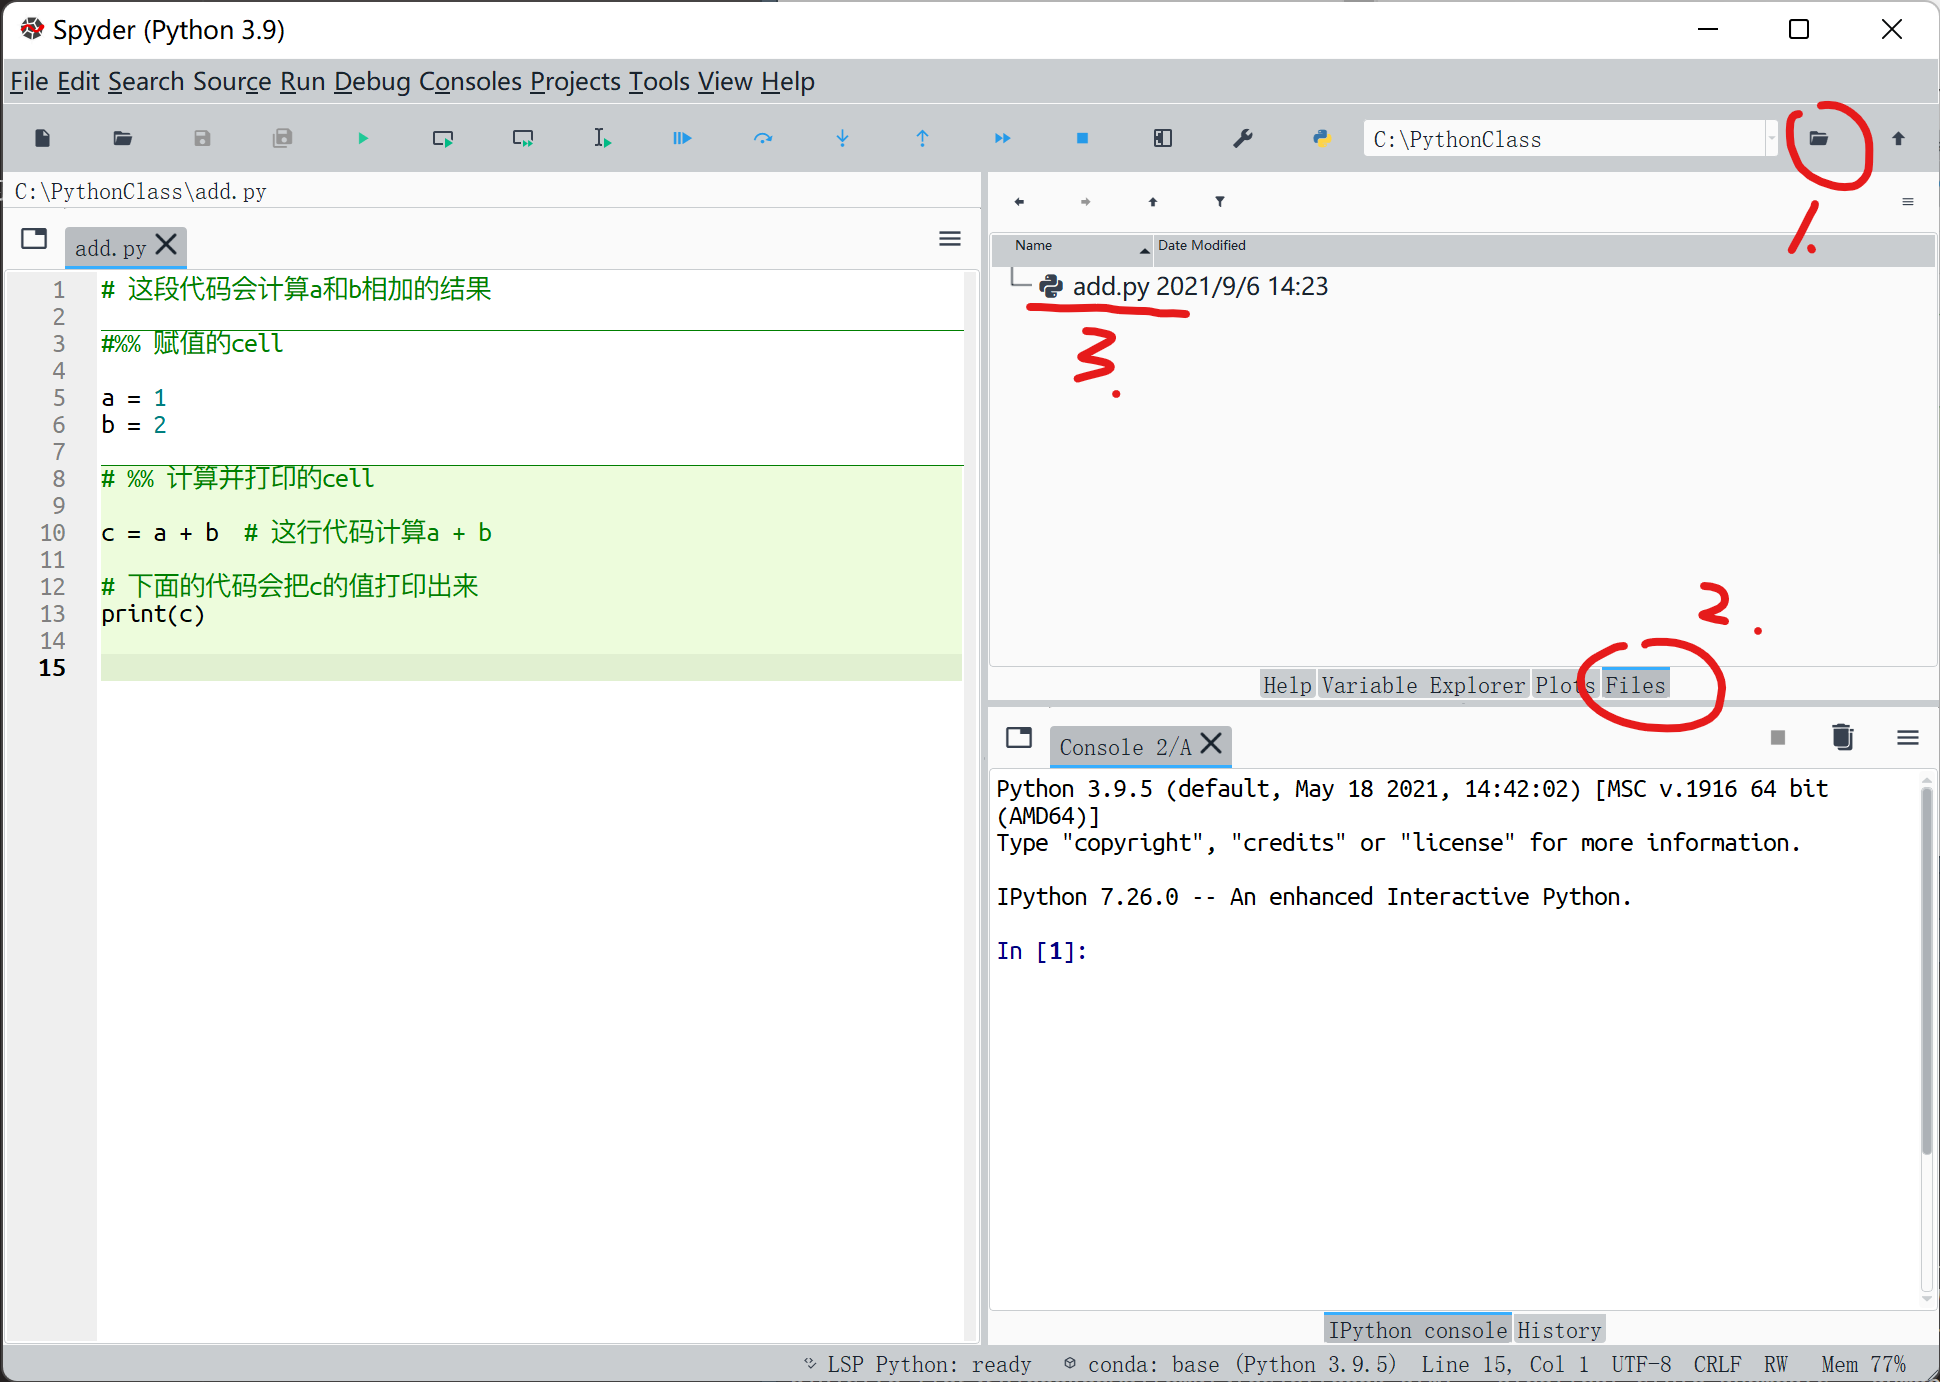
\includegraphics{images/btn_setwd.png}

\begin{enumerate}
\def\labelenumi{\arabic{enumi}.}
\setcounter{enumi}{1}
\tightlist
\item
  切换到Files标签栏
\item
  把我们正在编辑的py文件,另存为到工作目录,命名为\texttt{add.py}。这样,在文件列表,我们会看到这个文件
\end{enumerate}

注意:如果前面大家按步骤做,这里应该会覆盖掉上一节课的同名文件。

\hypertarget{ux53d8ux91cfux548cux5e38ux7528ux6570ux636eux7c7bux578b}{%
\chapter{变量和常用数据类型}\label{ux53d8ux91cfux548cux5e38ux7528ux6570ux636eux7c7bux578b}}

\hypertarget{ux53d8ux91cf}{%
\section{变量}\label{ux53d8ux91cf}}

前面说过,Python(或者其他编程语言)中的变量,和你数学课上的\texttt{x,\ y,\ z}是同类的概念。

正如前面的例子,Python使用等号\texttt{=}来为一个变量赋值

\begin{Shaded}
\begin{Highlighting}[]
\CommentTok{\#\%\% 赋值与重新赋值}
\NormalTok{a }\OperatorTok{=} \DecValTok{1}
\NormalTok{a }\OperatorTok{=} \DecValTok{2}
\NormalTok{a}
\end{Highlighting}
\end{Shaded}

假如这个一开始不存在,那么赋值的同时,也会把这个变量创造出来。

对于Python语言,这个过程(\textbf{不严格地说})大致是:

\begin{enumerate}
\def\labelenumi{\arabic{enumi}.}
\tightlist
\item
  (绑定)Python在电脑的内存空间找了一个空地,创建了一个对象(object),存放了\texttt{1}这个值,然后把\texttt{a}这个名字,和这个对象绑定起来。
\item
  (重绑定)当我们对变量\texttt{a}赋其他值的时候,如\texttt{a\ =\ 2}的时候,Python另外创建了一个对象,存放了\texttt{2}这个值,然后把\texttt{a}这个名字,重新绑定到这个新的对象上。
\item
  (引用)变量名,就像一个内存中的对象的标签。引用这个名字,就是引用其表示的对象。
\end{enumerate}

\hypertarget{ux5220ux9664ux4e00ux4e2aux53d8ux91cf}{%
\subsection{删除一个变量}\label{ux5220ux9664ux4e00ux4e2aux53d8ux91cf}}

使用del语句

\begin{Shaded}
\begin{Highlighting}[]
\CommentTok{\#\%\% 删除变量}
\NormalTok{a }\OperatorTok{=} \DecValTok{1}
\KeywordTok{del}\NormalTok{ a}
\NormalTok{a}
\end{Highlighting}
\end{Shaded}

因为变量\texttt{a}已经被我们删除了,所以你再次引用\texttt{a}的时候,Python会告诉你,

\begin{verbatim}
NameError: name 'a' is not defined
\end{verbatim}

\hypertarget{ux52a8ux6001ux8bedux8a00}{%
\subsection{动态语言}\label{ux52a8ux6001ux8bedux8a00}}

Python是一个``动态语言'',即Python的变量的类型是在运行过程中决定,或者说可以在运行中改变:你对这个变量赋什么值,这个变量就是什么类型。

查看变量类型的函数是\texttt{type()}

例如

\begin{Shaded}
\begin{Highlighting}[]
\CommentTok{\#\%\% 动态类型}
\NormalTok{a }\OperatorTok{=} \DecValTok{1} 
\BuiltInTok{print}\NormalTok{(}\BuiltInTok{type}\NormalTok{(a))}

\NormalTok{a }\OperatorTok{=} \StringTok{\textquotesingle{}apple\textquotesingle{}} \CommentTok{\# 这里为a赋值了一个字符串}
\BuiltInTok{print}\NormalTok{(}\BuiltInTok{type}\NormalTok{(a))}
\end{Highlighting}
\end{Shaded}

\begin{verbatim}
<class 'int'>
<class 'str'>
\end{verbatim}

显然,\texttt{a}先是一个整型int\texttt{\textless{}class\ \textquotesingle{}int\textquotesingle{}\textgreater{}},然后变成了一个字符串str\texttt{\textless{}class\ \textquotesingle{}str\textquotesingle{}\textgreater{}}。
这和我们的赋值顺序是一样的。类型后面会详细说

\textcolor{red}{**注意**:}Python的变量类型是动态确定的。变量的类型不一定能从名字看出来,这是出错的一大来源。

\hypertarget{ux53d8ux91cfux7684ux547dux540dux89c4ux5219}{%
\subsection{变量的命名规则}\label{ux53d8ux91cfux7684ux547dux540dux89c4ux5219}}

\hypertarget{ux6570ux503c}{%
\section{数值}\label{ux6570ux503c}}

Python 3.x以后,数值类型有2种,整型\texttt{int},和浮点型\texttt{float}。

顾名思义,整型可以理解为整数:

\begin{Shaded}
\begin{Highlighting}[]
\CommentTok{\#\%\% 整型}
\NormalTok{a }\OperatorTok{=} \DecValTok{1}
\BuiltInTok{type}\NormalTok{(a)}
\end{Highlighting}
\end{Shaded}

\begin{verbatim}
## <class 'int'>
\end{verbatim}

而浮点型则可以理解为小数:

\begin{Shaded}
\begin{Highlighting}[]
\CommentTok{\#\%\% 浮点型}
\NormalTok{a }\OperatorTok{=} \FloatTok{1.23}
\BuiltInTok{type}\NormalTok{(a)}
\end{Highlighting}
\end{Shaded}

\begin{verbatim}
## <class 'float'>
\end{verbatim}

特别地,\texttt{a\ =\ 1.0}是什么类型?

\begin{Shaded}
\begin{Highlighting}[]
\NormalTok{a }\OperatorTok{=} \FloatTok{1.0}
\BuiltInTok{type}\NormalTok{(a)}
\end{Highlighting}
\end{Shaded}

\begin{verbatim}
## <class 'float'>
\end{verbatim}

显然,\texttt{a}是浮点型:只要你赋值的时候有小数点。
这可能是因为:

\begin{enumerate}
\def\labelenumi{\arabic{enumi}.}
\tightlist
\item
  这个变量客观上是个小数,只是``恰好''是1而已。
\item
  或者这个数被四舍五入,比如本来是\texttt{1.0000001}之类。
\end{enumerate}

\hypertarget{ux6570ux503cux7684ux64cdux4f5c}{%
\subsection{数值的操作}\label{ux6570ux503cux7684ux64cdux4f5c}}

\begin{enumerate}
\def\labelenumi{\arabic{enumi}.}
\tightlist
\item
  常见的操作包括加减乘除\texttt{+,\ -,\ *,\ /},此处不再重复。
\end{enumerate}

特别地,除法永远返回浮点类型:

\begin{Shaded}
\begin{Highlighting}[]
\NormalTok{a }\OperatorTok{=} \DecValTok{4} \OperatorTok{/} \DecValTok{2}
\BuiltInTok{print}\NormalTok{(a)}
\end{Highlighting}
\end{Shaded}

\begin{verbatim}
## 2.0
\end{verbatim}

\begin{Shaded}
\begin{Highlighting}[]
\BuiltInTok{type}\NormalTok{(a)}
\end{Highlighting}
\end{Shaded}

\begin{verbatim}
## <class 'float'>
\end{verbatim}

\begin{enumerate}
\def\labelenumi{\arabic{enumi}.}
\setcounter{enumi}{1}
\tightlist
\item
  整除是\texttt{//}。若除数是整型,则返回整型;若出数是浮点型,则返回浮点型
\end{enumerate}

\begin{Shaded}
\begin{Highlighting}[]
\DecValTok{5} \OperatorTok{//} \DecValTok{2}
\end{Highlighting}
\end{Shaded}

\begin{verbatim}
## 2
\end{verbatim}

\begin{Shaded}
\begin{Highlighting}[]
\DecValTok{5} \OperatorTok{//} \FloatTok{2.0}
\end{Highlighting}
\end{Shaded}

\begin{verbatim}
## 2.0
\end{verbatim}

\begin{enumerate}
\def\labelenumi{\arabic{enumi}.}
\setcounter{enumi}{2}
\tightlist
\item
  取余\texttt{\%}
\end{enumerate}

\begin{Shaded}
\begin{Highlighting}[]
\DecValTok{5} \OperatorTok{\%} \DecValTok{2}
\end{Highlighting}
\end{Shaded}

\begin{verbatim}
## 1
\end{verbatim}

\begin{enumerate}
\def\labelenumi{\arabic{enumi}.}
\setcounter{enumi}{3}
\tightlist
\item
  乘方 \(2^3\)
\end{enumerate}

\begin{Shaded}
\begin{Highlighting}[]
\DecValTok{2} \OperatorTok{**} \DecValTok{3}
\end{Highlighting}
\end{Shaded}

\begin{verbatim}
## 8
\end{verbatim}

\hypertarget{ux5b57ux7b26ux4e32str}{%
\section{字符串Str}\label{ux5b57ux7b26ux4e32str}}

创建字符串,可以使用单引号、双引号、三单引号和三双引号。其中三引号可以多行定义字符串。

\begin{enumerate}
\def\labelenumi{\arabic{enumi}.}
\tightlist
\item
  字符串:可以使用单引号、双引号
\end{enumerate}

\begin{Shaded}
\begin{Highlighting}[]
\CommentTok{\#\%\% 字符串}
\NormalTok{a }\OperatorTok{=} \StringTok{\textquotesingle{}apple\textquotesingle{}} \CommentTok{\# 或者:a = "apple"}
\NormalTok{a}
\end{Highlighting}
\end{Shaded}

\begin{verbatim}
## 'apple'
\end{verbatim}

\begin{enumerate}
\def\labelenumi{\arabic{enumi}.}
\setcounter{enumi}{1}
\tightlist
\item
  多行字符串:可以使用三个单引号,或者三个双引号。
\end{enumerate}

\begin{Shaded}
\begin{Highlighting}[]
\NormalTok{a }\OperatorTok{=} \StringTok{\textquotesingle{}\textquotesingle{}\textquotesingle{}Hello }
\StringTok{World}
\StringTok{\textquotesingle{}\textquotesingle{}\textquotesingle{}}
\NormalTok{a}
\end{Highlighting}
\end{Shaded}

\hypertarget{ux5b57ux7b26ux4e32ux7684ux5e38ux7528ux64cdux4f5c}{%
\subsection{字符串的常用操作}\label{ux5b57ux7b26ux4e32ux7684ux5e38ux7528ux64cdux4f5c}}

\begin{enumerate}
\def\labelenumi{\arabic{enumi}.}
\tightlist
\item
\end{enumerate}

\begin{verbatim}
Hello
World
\end{verbatim}

\hypertarget{ux5b57ux7b26ux4e32ux683cux5f0fux5316}{%
\subsection{字符串格式化}\label{ux5b57ux7b26ux4e32ux683cux5f0fux5316}}

\hypertarget{ux5e03ux5c14ux578b}{%
\section{布尔型}\label{ux5e03ux5c14ux578b}}

\hypertarget{ux770bux61c2ux51faux9519ux4fe1ux606f}{%
\section{看懂出错信息}\label{ux770bux61c2ux51faux9519ux4fe1ux606f}}

\hypertarget{ux5217ux8868}{%
\section{列表}\label{ux5217ux8868}}

\hypertarget{ux5143ux7ec4}{%
\section{元组}\label{ux5143ux7ec4}}

\hypertarget{ux5b57ux5178}{%
\section{字典}\label{ux5b57ux5178}}

\hypertarget{ux7c7bux578bux63d0ux793atype-hints}{%
\section{类型提示Type Hints}\label{ux7c7bux578bux63d0ux793atype-hints}}

\end{document}
